\PassOptionsToPackage{unicode=true}{hyperref} % options for packages loaded elsewhere
\PassOptionsToPackage{hyphens}{url}
%
\documentclass[ignorenonframetext,]{beamer}
\setbeamertemplate{caption}[numbered]
\setbeamertemplate{caption label separator}{: }
\setbeamercolor{caption name}{fg=normal text.fg}
\beamertemplatenavigationsymbolsempty
\usepackage{lmodern}
\usepackage{amssymb,amsmath}
\usepackage{ifxetex,ifluatex}
\usepackage{fixltx2e} % provides \textsubscript
\ifnum 0\ifxetex 1\fi\ifluatex 1\fi=0 % if pdftex
  \usepackage[T1]{fontenc}
  \usepackage[utf8]{inputenc}
  \usepackage{textcomp} % provides euro and other symbols
\else % if luatex or xelatex
  \usepackage{unicode-math}
  \defaultfontfeatures{Ligatures=TeX,Scale=MatchLowercase}
\fi
% use upquote if available, for straight quotes in verbatim environments
\IfFileExists{upquote.sty}{\usepackage{upquote}}{}
% use microtype if available
\IfFileExists{microtype.sty}{%
\usepackage[]{microtype}
\UseMicrotypeSet[protrusion]{basicmath} % disable protrusion for tt fonts
}{}
\IfFileExists{parskip.sty}{%
\usepackage{parskip}
}{% else
\setlength{\parindent}{0pt}
\setlength{\parskip}{6pt plus 2pt minus 1pt}
}
\usepackage{hyperref}
\hypersetup{
            pdftitle={Statistics and the Medical Literature},
            pdfauthor={Dave Harrington},
            pdfborder={0 0 0},
            breaklinks=true}
\urlstyle{same}  % don't use monospace font for urls
\newif\ifbibliography
\usepackage{longtable,booktabs}
\usepackage{caption}
% These lines are needed to make table captions work with longtable:
\makeatletter
\def\fnum@table{\tablename~\thetable}
\makeatother
\usepackage{graphicx,grffile}
\makeatletter
\def\maxwidth{\ifdim\Gin@nat@width>\linewidth\linewidth\else\Gin@nat@width\fi}
\def\maxheight{\ifdim\Gin@nat@height>\textheight\textheight\else\Gin@nat@height\fi}
\makeatother
% Scale images if necessary, so that they will not overflow the page
% margins by default, and it is still possible to overwrite the defaults
% using explicit options in \includegraphics[width, height, ...]{}
\setkeys{Gin}{width=\maxwidth,height=\maxheight,keepaspectratio}
% Prevent slide breaks in the middle of a paragraph:
\widowpenalties 1 10000
\raggedbottom
\setbeamertemplate{part page}{
\centering
\begin{beamercolorbox}[sep=16pt,center]{part title}
  \usebeamerfont{part title}\insertpart\par
\end{beamercolorbox}
}
\setbeamertemplate{section page}{
\centering
\begin{beamercolorbox}[sep=12pt,center]{part title}
  \usebeamerfont{section title}\insertsection\par
\end{beamercolorbox}
}
\setbeamertemplate{subsection page}{
\centering
\begin{beamercolorbox}[sep=8pt,center]{part title}
  \usebeamerfont{subsection title}\insertsubsection\par
\end{beamercolorbox}
}
\AtBeginPart{
  \frame{\partpage}
}
\AtBeginSection{
  \ifbibliography
  \else
    \frame{\sectionpage}
  \fi
}
\AtBeginSubsection{
  \frame{\subsectionpage}
}
\setlength{\emergencystretch}{3em}  % prevent overfull lines
\providecommand{\tightlist}{%
  \setlength{\itemsep}{0pt}\setlength{\parskip}{0pt}}
\setcounter{secnumdepth}{0}

% set default figure placement to htbp
\makeatletter
\def\fps@figure{htbp}
\makeatother


\usepackage{amsmath,verbatim}

\usepackage{fancyvrb}
\usepackage{manfnt}
\usepackage[normalem]{ulem}

%\usepackage[colorlinks=true]{hyperref}

\mode<presentation>{\usetheme{Malmoe}}

%\synctex=1

\setbeamertemplate{headline}{}


\setbeamerfont{footline}{size=\scriptsize}
\setbeamerfont{frametitle}{shape=\scshape}
\setbeamertemplate{itemize items}[circle]
\setbeamercovered{transparent}

\setbeamertemplate{navigation symbols}{}
\setbeamertemplate{footline}[frame number]{} 


\definecolor{forest}{rgb}{0, .5, 0}
\definecolor{brick}{rgb}{.5, 0, 0}
\definecolor{darkgreen}{rgb}{0, .5, 0}
\definecolor{darkred}{rgb}{.7, .15, .15}
\definecolor{darkblue}{rgb}{0, 0, .5}
\definecolor{Green}{rgb}{0.2,1,0.2}


\newcommand{\R}{\textsf{R}}
\newcommand{\RStudio}{\textsl{R Studio}}


\usepackage[english]{babel}
%\usepackage{palatino}
\usepackage[T1]{fontenc}


% make all tt fonts bold to look more like Verbatim
\usepackage{lmodern}
\renewcommand\ttfamily{\usefont{T1}{lmtt}{m}{n}}

% Comment these out if you don't want a slide with just the
% part/section/subsection/subsubsection title:
\AtBeginPart{
  \let\insertpartnumber\relax
  \let\partname\relax
  \frame{\partpage}
}
\AtBeginSection{
  \let\insertsectionnumber\relax
 \let\sectionname\relax
 \frame{\sectionpage}
}
\AtBeginSubsection{
  \let\insertsubsectionnumber\relax
  \let\subsectionname\relax
  \frame{\subsectionpage}
}

\logo{
\includegraphics[width=.50\textwidth]{DFCI_DDS_Logo.png}\hspace*{.55\paperwidth}\vspace*{-.2in}}
\newcommand{\nologo}{\setbeamertemplate{logo}{}} % command to set the logo to nothing

\title{Statistics and the Medical Literature}
\author{Dave Harrington}
\date{11 October 2019}

\begin{document}
\frame{\titlepage}

\begin{frame}
\tableofcontents[hideallsubsections]
\end{frame}
\hypertarget{interpreting-study-design-and-analysis}{%
\section{Interpreting study design and
analysis}\label{interpreting-study-design-and-analysis}}

\begin{frame}{%
\protect\hypertarget{main-elements-of-the-design-rcts-and-observational-studies}{%
Main elements of the design – RCTs and observational studies}}

Plan to minimize bias?

\begin{itemize}
\item
  RCT: Randomization, blinding, identical evaluation/follow-up schedules
\item
  Observational studies: record important confounders, plan for post-hoc
  adjustment, perhaps include matching in recruitment
\end{itemize}

Chance of detecting important effects/associations? (Adequately powered,
at least 80\%) \medskip

Plan to minimize false positive results if many endpoints/subgroups
examined?

\begin{itemize}
\tightlist
\item
  More difficult with large observational studies, especially
  genomics/genetics
\end{itemize}

\end{frame}

\begin{frame}{%
\protect\hypertarget{power-and-type-i-error}{%
Power and type I error}}

Type I error (alpha error)

\begin{itemize}
\item
  Probability that trial will report a false positive, i.e., claim a
  significant result when there is no treatment effect.
\item
  Typically set no larger than 5\%
\item
  Depends on method of analysis, does not depend on sample size
\end{itemize}

\end{frame}

\begin{frame}{%
\protect\hypertarget{power}{%
Power}}

\begin{itemize}
\item
  Probability that the trial will report a true positive, i.e., claim a
  significant result when there is a treatment effect.
\item
  Should be 80\% or greater
\item
  Depends on sample size, method of analysis and size of treatment
  effect.
\item
  Power calculations relevant when study is designed.
\item
  Power calculations have little value after a study is complete.

  \begin{itemize}
  \tightlist
  \item
    Precision measured through confidence intervals
  \end{itemize}
\end{itemize}

\end{frame}

\begin{frame}{%
\protect\hypertarget{design-of-sprint-nejm-26-nov-2015}{%
Design of SPRINT (NEJM 26 Nov 2015)}}

From the methods section of the paper:

\begin{quote}
We planned a 2-year recruitment period, with a maximum follow-up of 6 years, and anticipated a loss to follow-up of 2\% per year. With an enrollment target of 9250 participants, we estimated  that the trial would have 88.7\% power to detect  a 20\% effect with respect to the primary outcome, assuming an event rate of 2.2\% in the standard-treatment group.
\end{quote}

\end{frame}

\begin{frame}{%
\protect\hypertarget{calculating-power}{%
Calculating Power}}

Next two slides show graphs of power in hypothetical study of a blood
pressure lowering medication. \medskip

Two medications, experimental vs control, using \(\alpha = 0.05\)

\begin{itemize}
\item
  First, power as a function of sample size if true effect is 3mmHg
  reduction
\item
  Second, power as a function of reduction in bp (effect size) for
  sample size 250 per group.
\end{itemize}

\end{frame}

\begin{frame}{%
\protect\hypertarget{power-vs.sample-size}{%
Power vs.~sample size}}

\small

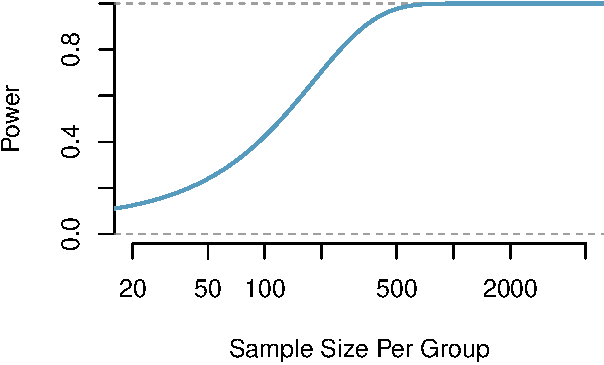
\includegraphics{med_student_2019_files/figure-beamer/power_sample-1.pdf}

More than about 250 to 350 per group doesn’t provide much additional
value.

\end{frame}

\begin{frame}{%
\protect\hypertarget{power-vs.effect-size-250-participants-per-group}{%
Power vs.~effect size, 250 participants per group}}

\small

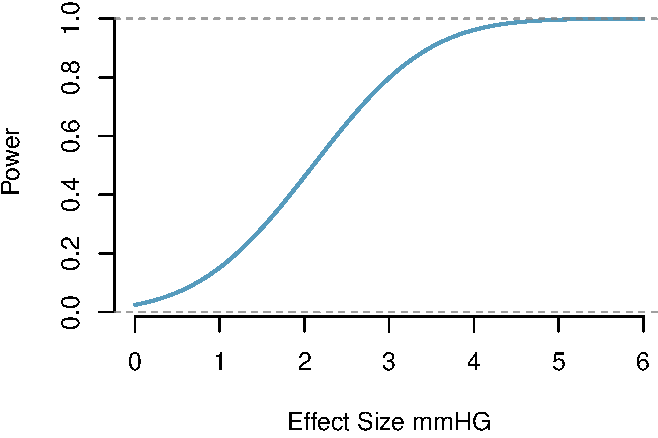
\includegraphics{med_student_2019_files/figure-beamer/power_effect-1.pdf}

\end{frame}

\begin{frame}{%
\protect\hypertarget{confidence-intervals}{%
Confidence intervals}}

Confidence intervals are the preferred way to summarize outcome data,
and are more informative post-hoc than power calculations. \medskip

Easiest definition:

\begin{itemize}
\item
  Confidence interval provides a single estimate with a `margin of
  error’.
\item
  The size of the margin is determined by the variability in the data
  and the `confidence coefficient’
\end{itemize}

Confidence coefficient is the proportion of times (in repeated sampling)
an interval will contain the true treatment effect.

\end{frame}

\begin{frame}{%
\protect\hypertarget{measuring-precision-after-study-completion}{%
Measuring precision after study completion}}

From
\textit{Postmenopausal estrogen use and progestin use and the risk of cardiovascular disease,}
NEJM 15 August 1996

\begin{quote}
We observed a marked decrease in the risk of major coronary heart disease among women who took estrogen with progestin, as compared with the risk among women who did not use hormones (multivariate adjusted relative risk, 0.39; 95 percent confidence interval, 0.19 to 0.78) \ldots
\end{quote}

\end{frame}

\begin{frame}{%
\protect\hypertarget{measuring-precision-after-study-completion-1}{%
Measuring precision after study completion}}

\begin{quote}
However, there was no significant association between stroke and use of combined hormones (multivariate adjusted relative risk, 1.09; 95 percent confidence interval, 0.66 to 1.80) \ldots

\end{quote}

\end{frame}

\begin{frame}{%
\protect\hypertarget{controlling-type-i-error}{%
Controlling type I error}}

\small

The more tests one does, the more likely it is that \emph{at least one}
will be a false positive. \medskip

Suppose each test is done at level \(\alpha = 0.05\).

\begin{longtable}[]{@{}cc@{}}
\toprule
\begin{minipage}[b]{0.34\columnwidth}\centering
Number of Comparisons\strut
\end{minipage} & \begin{minipage}[b]{0.38\columnwidth}\centering
Experimentwise Error\strut
\end{minipage}\tabularnewline
\midrule
\endhead
\begin{minipage}[t]{0.34\columnwidth}\centering
1\strut
\end{minipage} & \begin{minipage}[t]{0.38\columnwidth}\centering
0.05\strut
\end{minipage}\tabularnewline
\begin{minipage}[t]{0.34\columnwidth}\centering
2\strut
\end{minipage} & \begin{minipage}[t]{0.38\columnwidth}\centering
0.10\strut
\end{minipage}\tabularnewline
\begin{minipage}[t]{0.34\columnwidth}\centering
3\strut
\end{minipage} & \begin{minipage}[t]{0.38\columnwidth}\centering
0.14\strut
\end{minipage}\tabularnewline
\begin{minipage}[t]{0.34\columnwidth}\centering
5\strut
\end{minipage} & \begin{minipage}[t]{0.38\columnwidth}\centering
0.23\strut
\end{minipage}\tabularnewline
\begin{minipage}[t]{0.34\columnwidth}\centering
10\strut
\end{minipage} & \begin{minipage}[t]{0.38\columnwidth}\centering
0.40\strut
\end{minipage}\tabularnewline
\begin{minipage}[t]{0.34\columnwidth}\centering
100\strut
\end{minipage} & \begin{minipage}[t]{0.38\columnwidth}\centering
\textgreater{}0.90\strut
\end{minipage}\tabularnewline
\bottomrule
\end{longtable}

Experimentwise error: at least one positive result when there are no
treatment effects.

Dangerous in the analysis of subgroups.

\end{frame}

\begin{frame}{%
\protect\hypertarget{controlling-type-1-error}{%
Controlling type 1 error}}

Assume target experimentwise error 5\% (\(\alpha =0.05\)) \medskip

Bonferroni approximation, no order specified for comparisons

\begin{itemize}
\item
  Divide significance level by number of planned tests
\item
  5 comparisons, use p = 0.01
\item
  Not practical when many comparisons planned, especially in genetics
  studies
\end{itemize}

\end{frame}

\begin{frame}{%
\protect\hypertarget{controlling-type-1-error-1}{%
Controlling type 1 error\ldots}}

Holm’s method, no order specified

\begin{itemize}
\item
  Order the p-values from smallest to largest
\item
  Stop testing as soon as a p-value is too large
\item
  5 comparisons:

  \begin{itemize}
  \item
    Compare smallest p-value to 0.05/5 = 0.01.
  \item
    Compare next smallest to 0.05/4 = 0.0125.
  \item
    Next smallest to 0.05/3
  \item
    etc
  \end{itemize}
\end{itemize}

\end{frame}

\hypertarget{special-topic-what-happens-when-there-is-attrition}{%
\section{Special topic: What happens when there is
attrition?}\label{special-topic-what-happens-when-there-is-attrition}}

\begin{frame}{%
\protect\hypertarget{problems-caused-by-attrition}{%
Problems caused by attrition}}

Attrition in an RCT can cause several problems

\begin{itemize}
\item
  Random attrition reduces effective sample size
\item
  Missing data from non-random attrition can cause bias
\end{itemize}

Two strategies in general use:

\begin{itemize}
\item
  Intent-to-treat (ITT)
\item
  Per protocol (PP)
\end{itemize}

Neither is perfect

\end{frame}

\begin{frame}{%
\protect\hypertarget{intent-to-treat-itt-vs.per-protocol-pp}{%
Intent-to-treat (ITT) vs.~per-protocol (PP)}}

ITT: analyze according to assigned treatment, not treatment received.
\medskip

Main justification:

\begin{itemize}
\item
  p-values are calculated assuming no treatment difference (the null
  hypothesis)
\item
  Under that assumption, assigned treatment does not affect outcome.
\item
  p-values will be correct (valid) when comparing the two groups
  according to treatment assignment.
\end{itemize}

Example may help make this clear.

\end{frame}

\begin{frame}{%
\protect\hypertarget{simple-trial-success-vs-failure-outcome-no-difference-non-random-crossover}{%
Simple trial, success vs failure outcome, no difference, non-random
crossover}}

\small

Suppose two treatments (\(A\) and \(B\)) are equally effective.

100 participants randomized to each treatment.

ITT table:

\begin{longtable}[]{@{}ccc@{}}
\toprule
\begin{minipage}[b]{0.15\columnwidth}\centering
Response\strut
\end{minipage} & \begin{minipage}[b]{0.22\columnwidth}\centering
Treatment \(A\)\strut
\end{minipage} & \begin{minipage}[b]{0.25\columnwidth}\centering
Treatment \(B\)\strut
\end{minipage}\tabularnewline
\midrule
\endhead
\begin{minipage}[t]{0.15\columnwidth}\centering
Success\strut
\end{minipage} & \begin{minipage}[t]{0.22\columnwidth}\centering
40\strut
\end{minipage} & \begin{minipage}[t]{0.25\columnwidth}\centering
40\strut
\end{minipage}\tabularnewline
\begin{minipage}[t]{0.15\columnwidth}\centering
Failure\strut
\end{minipage} & \begin{minipage}[t]{0.22\columnwidth}\centering
60\strut
\end{minipage} & \begin{minipage}[t]{0.25\columnwidth}\centering
60\strut
\end{minipage}\tabularnewline
\bottomrule
\end{longtable}

Now assume, after randomization:

\begin{itemize}
\item
  10 participants with good prognosis (future responders) switch from
  \(A\) to \(B\)
\item
  10 participants with bad prognosis (future non-responders) switch from
  \(B\) to \(A\)
\end{itemize}

\end{frame}

\begin{frame}{%
\protect\hypertarget{simple-trial-but-with-selective-crossovers.}{%
Simple trial, but with selective crossovers.}}

Two treatments still equally effective.

Table for the as-treated groups

\begin{longtable}[]{@{}ccc@{}}
\toprule
\begin{minipage}[b]{0.15\columnwidth}\centering
Response\strut
\end{minipage} & \begin{minipage}[b]{0.22\columnwidth}\centering
Treatment \(A\)\strut
\end{minipage} & \begin{minipage}[b]{0.25\columnwidth}\centering
Treatment \(B\)\strut
\end{minipage}\tabularnewline
\midrule
\endhead
\begin{minipage}[t]{0.15\columnwidth}\centering
Success\strut
\end{minipage} & \begin{minipage}[t]{0.22\columnwidth}\centering
30\strut
\end{minipage} & \begin{minipage}[t]{0.25\columnwidth}\centering
50\strut
\end{minipage}\tabularnewline
\begin{minipage}[t]{0.15\columnwidth}\centering
Failure\strut
\end{minipage} & \begin{minipage}[t]{0.22\columnwidth}\centering
70\strut
\end{minipage} & \begin{minipage}[t]{0.25\columnwidth}\centering
50\strut
\end{minipage}\tabularnewline
\bottomrule
\end{longtable}

An as-treated analysis would imply \(B\) more effective than \(A\)

\end{frame}

\begin{frame}{%
\protect\hypertarget{itt-can-be-biased-when-there-is-a-real-treatment-effect-random-crossovers}{%
ITT can be biased when there is a real treatment effect (random
crossovers)}}

\small

Suppose \(B\) is more effective than \(A\), so for 100 in each group:

\begin{longtable}[]{@{}ccc@{}}
\toprule
\begin{minipage}[b]{0.15\columnwidth}\centering
Response\strut
\end{minipage} & \begin{minipage}[b]{0.22\columnwidth}\centering
Treatment \(A\)\strut
\end{minipage} & \begin{minipage}[b]{0.25\columnwidth}\centering
Treatment \(B\)\strut
\end{minipage}\tabularnewline
\midrule
\endhead
\begin{minipage}[t]{0.15\columnwidth}\centering
Success\strut
\end{minipage} & \begin{minipage}[t]{0.22\columnwidth}\centering
30\strut
\end{minipage} & \begin{minipage}[t]{0.25\columnwidth}\centering
50\strut
\end{minipage}\tabularnewline
\begin{minipage}[t]{0.15\columnwidth}\centering
Failure\strut
\end{minipage} & \begin{minipage}[t]{0.22\columnwidth}\centering
70\strut
\end{minipage} & \begin{minipage}[t]{0.25\columnwidth}\centering
50\strut
\end{minipage}\tabularnewline
\bottomrule
\end{longtable}

Assume 10 randomly chosen participants from each group switch
treatments, after randomization but before starting treatment.

\end{frame}

\begin{frame}{%
\protect\hypertarget{table-with-just-patients-who-do-not-switch}{%
Table with just patients who do not switch}}

\begin{longtable}[]{@{}ccc@{}}
\toprule
\begin{minipage}[b]{0.15\columnwidth}\centering
Response\strut
\end{minipage} & \begin{minipage}[b]{0.22\columnwidth}\centering
Treatment \(A\)\strut
\end{minipage} & \begin{minipage}[b]{0.25\columnwidth}\centering
Treatment \(B\)\strut
\end{minipage}\tabularnewline
\midrule
\endhead
\begin{minipage}[t]{0.15\columnwidth}\centering
Success\strut
\end{minipage} & \begin{minipage}[t]{0.22\columnwidth}\centering
27\strut
\end{minipage} & \begin{minipage}[t]{0.25\columnwidth}\centering
45\strut
\end{minipage}\tabularnewline
\begin{minipage}[t]{0.15\columnwidth}\centering
Failure\strut
\end{minipage} & \begin{minipage}[t]{0.22\columnwidth}\centering
63\strut
\end{minipage} & \begin{minipage}[t]{0.25\columnwidth}\centering
45\strut
\end{minipage}\tabularnewline
\bottomrule
\end{longtable}

Attrition did not change measured success rates

\begin{itemize}
\tightlist
\item
  but it does reduce the effective sample size
\end{itemize}

What happens when `switchers’ are put back in?

\begin{itemize}
\item
  10 \(A\) \(\rightarrow\) \(B\), 5 respond, 5 do not
\item
  10 \(B\) \(\rightarrow\) \(A\), 3 respond, 7 do not
\end{itemize}

\end{frame}

\begin{frame}{%
\protect\hypertarget{itt-table-with-assigned-treatment-real-response}{%
ITT Table with assigned treatment, real response}}

\small

\(A\) gets 5 responders (who received B)

\(B\) gets 3 responders (who received A)

\begin{longtable}[]{@{}ccc@{}}
\toprule
\begin{minipage}[b]{0.15\columnwidth}\centering
Response\strut
\end{minipage} & \begin{minipage}[b]{0.22\columnwidth}\centering
Treatment \(A\)\strut
\end{minipage} & \begin{minipage}[b]{0.25\columnwidth}\centering
Treatment \(B\)\strut
\end{minipage}\tabularnewline
\midrule
\endhead
\begin{minipage}[t]{0.15\columnwidth}\centering
Success\strut
\end{minipage} & \begin{minipage}[t]{0.22\columnwidth}\centering
32\strut
\end{minipage} & \begin{minipage}[t]{0.25\columnwidth}\centering
48\strut
\end{minipage}\tabularnewline
\begin{minipage}[t]{0.15\columnwidth}\centering
Failure\strut
\end{minipage} & \begin{minipage}[t]{0.22\columnwidth}\centering
68\strut
\end{minipage} & \begin{minipage}[t]{0.25\columnwidth}\centering
52\strut
\end{minipage}\tabularnewline
\bottomrule
\end{longtable}

Apparent success rate:\\
- \(A\) 32\% vs.~30\% after vs.~before crossover - \(B\) 48\% vs.~50\%
after vs.~before crossover

Response proportions have moved closer together.

Non-random attrition can also cause bias in the analysis because of
missing data

\end{frame}

\hypertarget{special-topic-non-inferiority-ni-trials}{%
\section{Special Topic: Non-inferiority (NI)
trials}\label{special-topic-non-inferiority-ni-trials}}

\begin{frame}{%
\protect\hypertarget{goals-of-ni-trials}{%
Goals of NI trials}}

\(T\) = experimental treatment; \(C\) = active control

The NI design has one explicit and one implicit goal.

\begin{itemize}
\tightlist
\item
  Explicit goal: demonstrate that \(T\) is as effective, or nearly as
  effective, as best available therapy, \(C\).\\
\item
  Implicit goal: demonstrate that \(T\) is better than placebo or no
  treatment (labeled \(P\) for placebo).
\end{itemize}

Ordinarily, both must be true for \(T\) to be a therapeutic option.

\end{frame}

\begin{frame}{%
\protect\hypertarget{goals-of-ni-designs}{%
Goals of NI Designs}}

The ideal study design would be a three-arm design, with \(P\), \(C\),
and \(T\).

But a placebo or no treatment arm is usually unethical

The non-inferiority trial provides a direct comparison of \(T\) to
\(C\), but it does not provide a direct comparison of \(T\) to \(P\).

\end{frame}

\begin{frame}{%
\protect\hypertarget{the-role-of-uncertainty-in-ni-trials}{%
The role of uncertainty in NI Trials}}

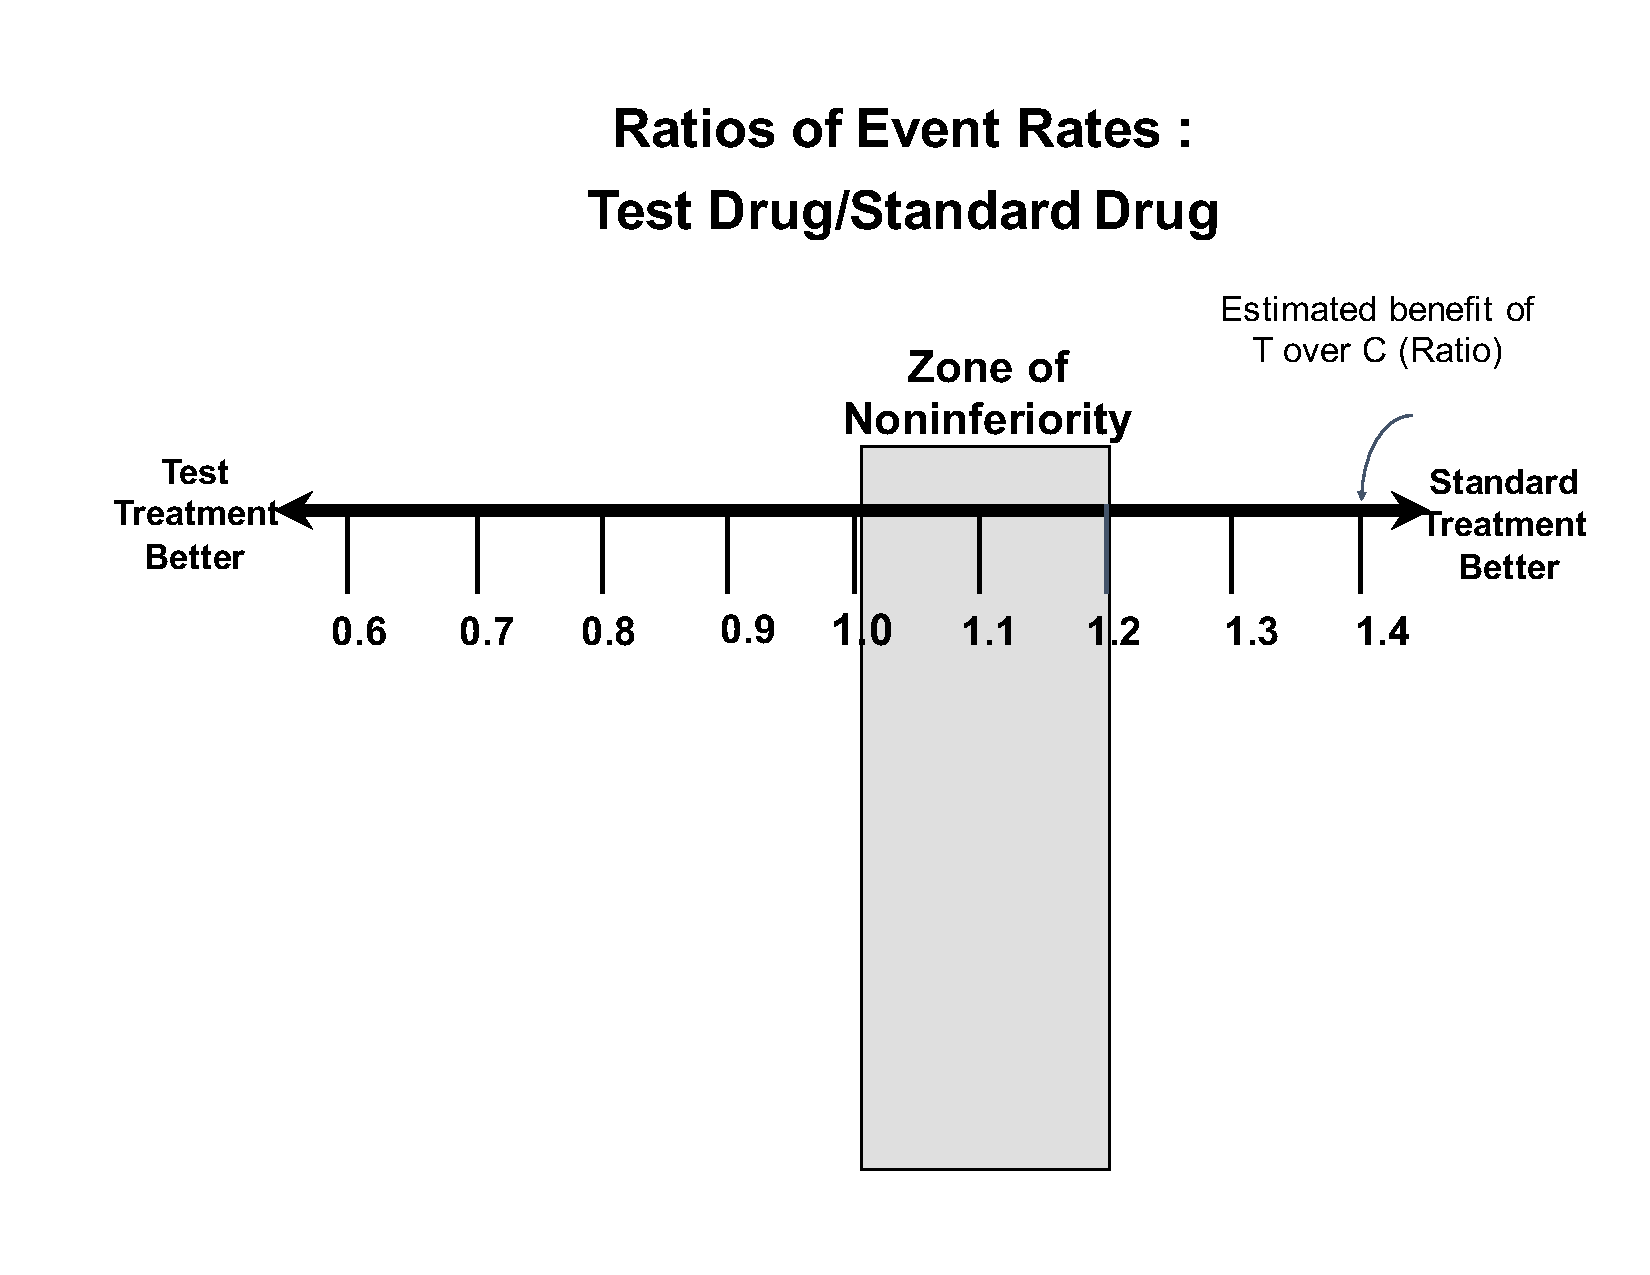
\includegraphics{ni_ci_rr_empty.pdf}

\end{frame}

\begin{frame}{%
\protect\hypertarget{section}{%
}}

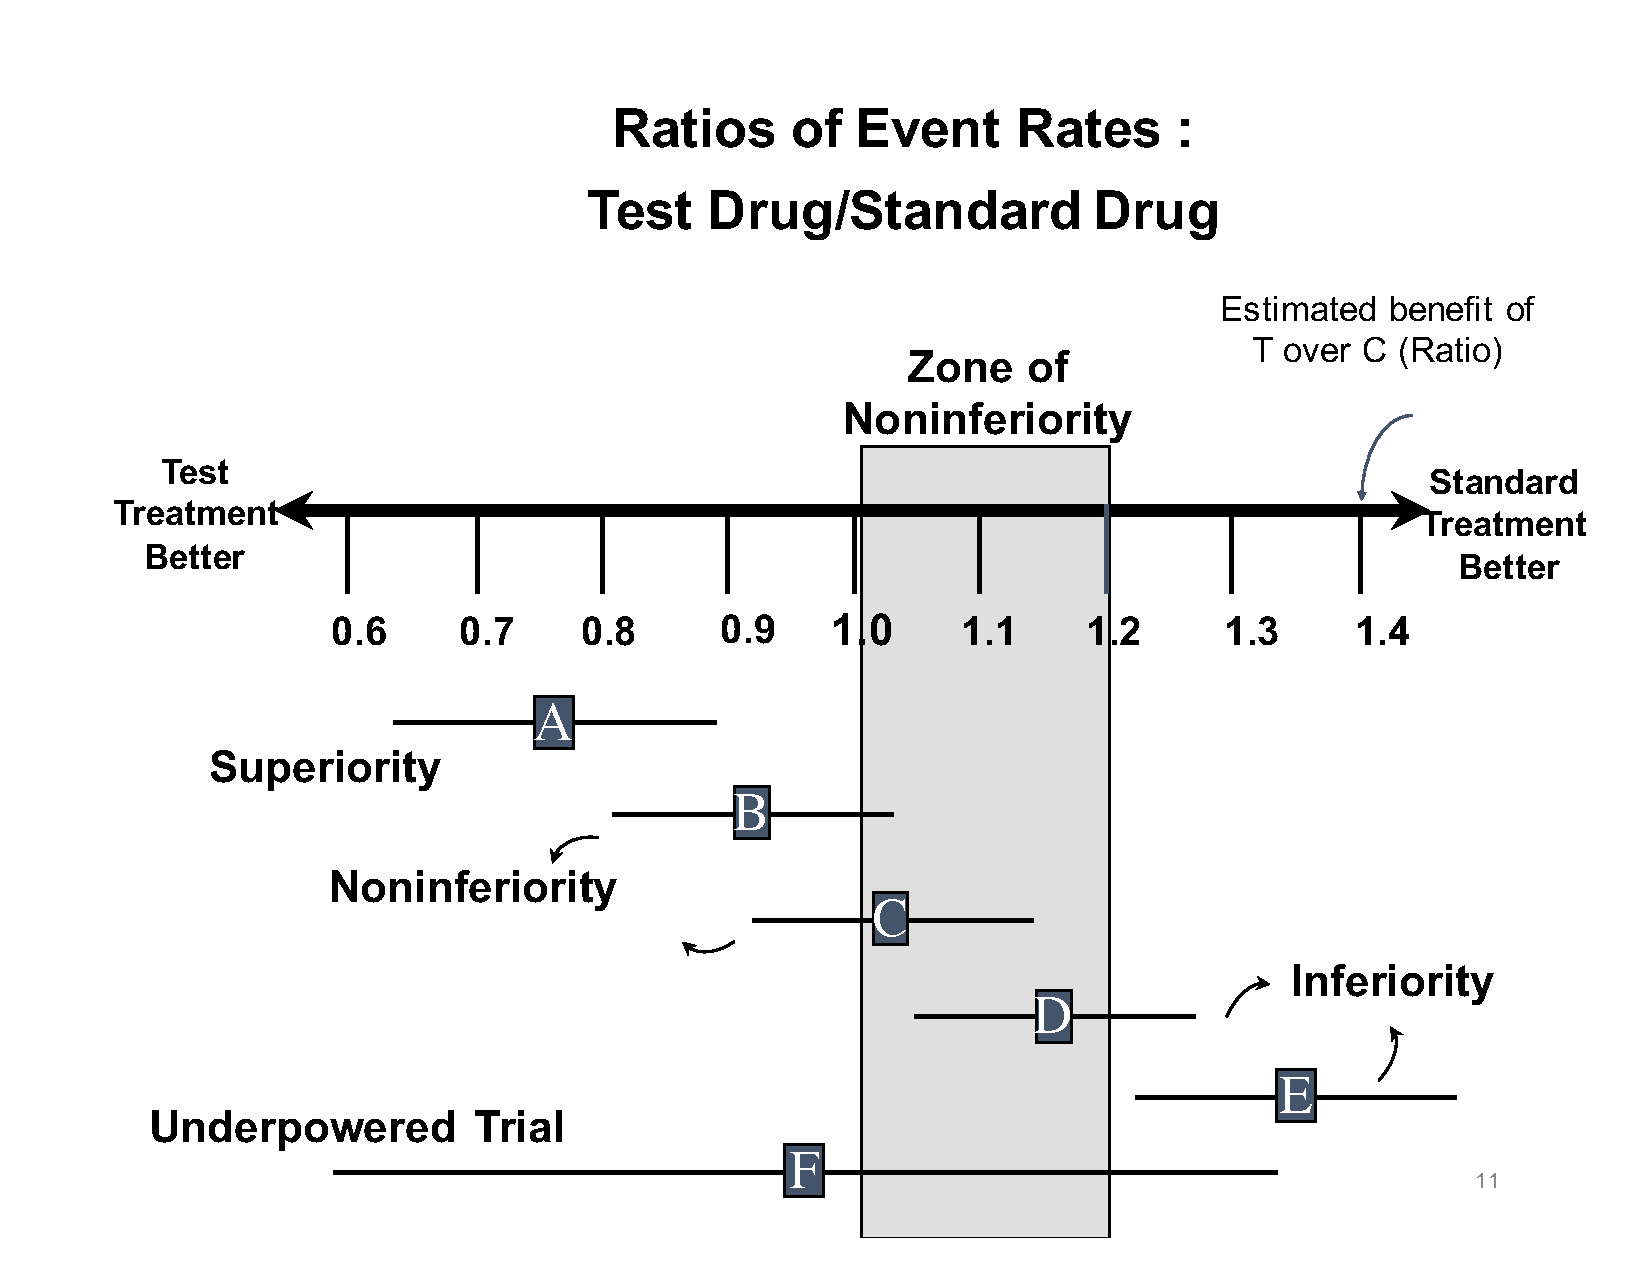
\includegraphics{ni_ci_rr_full.pdf}

\end{frame}

\begin{frame}{%
\protect\hypertarget{important-issues-in-analysis-of-ni-trials}{%
Important issues in analysis of NI Trials}}

The role of null and alternative hypotheses are reversed in NI trials.

Suppose on relative risk scale, the hazard ratio of Treatment vs control
should be no larger than 1.20

\begin{itemize}
\item
  The null hypothesis (\(H_0\)) is: Relative Risk \(\ge 1.20\)
\item
  The alternative hypothesis (\(H_A\)) is: Relative Risk \(< 1.20\)
\end{itemize}

Small \(p\)-values lead to rejection of \(H_0\)

\begin{itemize}
\tightlist
\item
  Small \(p\)-values are not evidence of a treatment difference.
\end{itemize}

Sample size should provide adequate power (at least 80\%) to reject
\(H_0\).

\end{frame}

\begin{frame}{%
\protect\hypertarget{issues-in-the-analysis-of-ni-trials}{%
Issues in the analysis of NI trials}}

Features of a trial which may lead to treatment differences appearing
smaller may inappropriately lead to claim of NI.

\begin{itemize}
\tightlist
\item
  Crossovers, non-adherence, subsets of patients for whom \(T\) or \(C\)
  is not likely to be effective
\end{itemize}

Intent to Treat analysis (ITT) may be biased in NI trials.

Safest to provide both

\begin{itemize}
\item
  ITT analyses
\item
  Per protocol (PP) analyses
\end{itemize}

\end{frame}

\begin{frame}{%
\protect\hypertarget{threats-to-validity-of-ni-designs}{%
Threats to Validity of NI Designs}}

Non-inferiority studies have some intrinsic limitations that make them
more difficult to design and more vulnerable to problems than the
superiority trials. \medskip

The following are the most important issues:

\begin{itemize}
\item
  Assay Sensitivity: possibility that \(T\) and \(C\) are ineffective,
  possibly from lack of adherence
\item
  Assay Constancy: \(C\) is still as effective as in historical trials
\item
  Dropouts can make two treatments seem more similar than they are.
\end{itemize}

\end{frame}

\begin{frame}{%
\protect\hypertarget{questions-to-ask-about-ni-trials}{%
Questions to ask about NI trials}}

\begin{itemize}
\item
  Is the claim of NI supported by a biological rationale?
\item
  Might the effect of Active Control (vs placebo) have been different in
  current trial?

  \begin{itemize}
  \tightlist
  \item
    Changes in administration of agent,\\
  \item
    Differences in populations using the drug or in endpoint
    determination
  \end{itemize}
\item
  Has long term follow-up changed the thinking of the value of the
  active control?
\item
  Does the analysis use the best available historical data on active
  control to estimate both treatment effects and uncertainty in the
  estimate?
\end{itemize}

\end{frame}

\begin{frame}{%
\protect\hypertarget{questions-to-ask-about-ni-trials-1}{%
Questions to ask about NI trials\ldots{}}}

\begin{itemize}
\item
  Is an estimated NI margin clinically relevant? Was it specified in
  advance of the analysis?
\item
  Is a reduced therapeutic effect for the test agent balanced by other
  benefits?
\item
  What is the margin of error (confidence interval) in the estimate of
  possible loss of efficacy?
\item
  Are results consistent across related endpoints?
\item
  As in all trials, treatment effects measured in NI analyses are
  estimates of population effects, not predictions of efficacy for
  individuals Is there a clear signal to the treating clinician on when
  to use the active control vs the new treatment?
\end{itemize}

\end{frame}

\hypertarget{the-buzz-about-p-values}{%
\section{\texorpdfstring{The buzz about
\(p\)-values}{The buzz about p-values}}\label{the-buzz-about-p-values}}

\begin{frame}{%
\protect\hypertarget{p-values-in-medical-literature}{%
P-values in medical literature}}

\(p < 0.05\) proposed by Fisher (1926) for single comparisons in
randomized experiments:

\begin{quote}

The value for which $P = 0.05$, or 1 in 20, is 1.96 or nearly 2; it is convenient to take this point as a limit in judging whether a deviation ought to be considered significant or not. 

\end{quote}

A \(p\)-value measures how much the observed data disagree with a
hypothesis of no treatment effect.

It is sometimes incorrectly interpreted as a measure of the
reproducibility of a trial

\begin{itemize}
\tightlist
\item
  or \(p < 0.05\) implies that the chance that the intervention works is
  at least 95\%
\end{itemize}

\end{frame}

\begin{frame}{%
\protect\hypertarget{analogy-with-diagnostic-testing}{%
Analogy with diagnostic testing}}

In a hypothesis test

Power of the test is likelihood of detecting a true effect

\begin{itemize}
\tightlist
\item
  \textcolor{darkblue}{Sensitivity}
\end{itemize}

Significance level of a test is the chance of test being positive when
effect is null

\begin{itemize}
\tightlist
\item
  It is the false positive rate, or
  \textcolor{darkblue}{1 - Specificity}
\end{itemize}

The positive predictive value of a hypothesis test is the chance the
intervention is effective when the test is statistically significant

\end{frame}

\begin{frame}{%
\protect\hypertarget{prevalence-affects-false-positive-rate}{%
Prevalence affects false positive rate}}

Next slide shows a graph of
\textcolor{darkblue}{probability of a false positive} conclusion in
favor of an intervention after a
\textcolor{darkblue}{statistically significant} result, based on

\begin{itemize}
\item
  Power of the study
\item
  Significance level threshold
\item
  \textcolor{forest}{Prior odds of a treatment effect}
\end{itemize}

\end{frame}

\begin{frame}{%
\protect\hypertarget{false-positive-probability-p-value-power-nat.-human-behavior-jan-2018}{%
False positive probability, p-value, power (Nat. Human Behavior, Jan
2018)}}

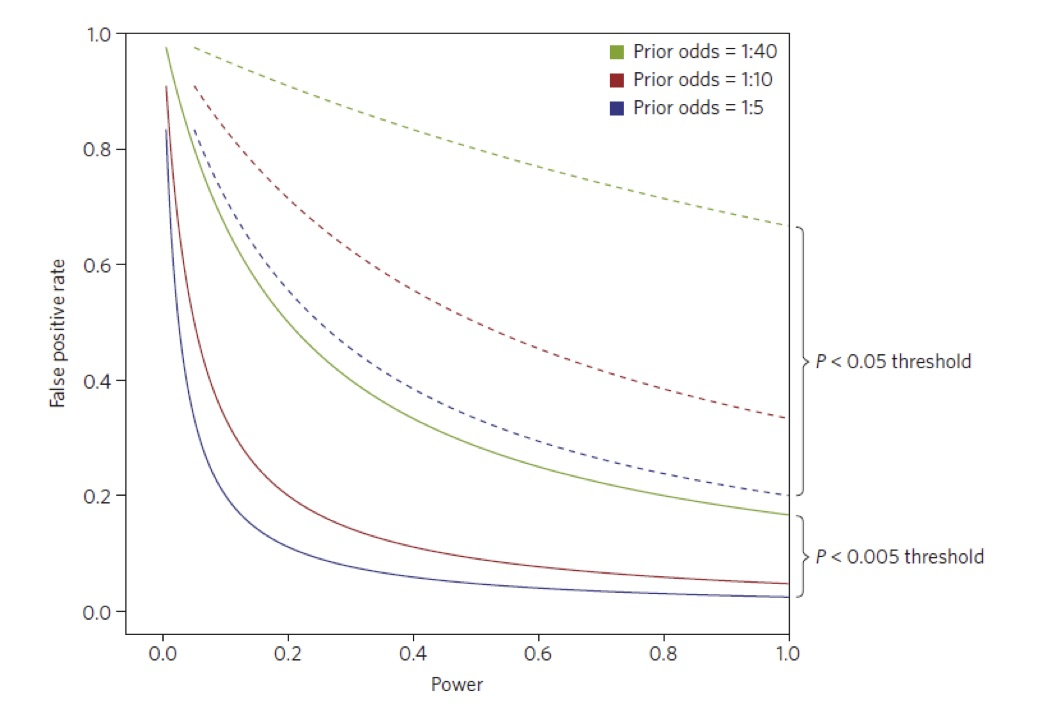
\includegraphics[width=1\textwidth,height=\textheight]{ppv_threshold.jpeg}

\end{frame}

\begin{frame}{%
\protect\hypertarget{what-if-the-actual-threshold-for-a-significant-result-is-larger-than-0.05}{%
What if the actual threshold for a ‘significant’ result is larger than
0.05?}}

\begin{longtable}[]{@{}llll@{}}
\toprule
Alpha & Prior Odds & Prob Null & False Pos. Prob\tabularnewline
\midrule
\endhead
0.1 & 1:5 & 0.83 & 0.38\tabularnewline
0.1 & 1:10 & 0.91 & 0.56\tabularnewline
0.1 & 1:40 & 0.98 & 0.83\tabularnewline
0.25 & 1:5 & 0.83 & 0.61\tabularnewline
0.25 & 1:10 & 0.91 & 0.76\tabularnewline
0.25 & 1:40 & 0.98 & 0.93\tabularnewline
\bottomrule
\end{longtable}

False Pos. Prob = probability of incorrectly claiming alternative is
true, given data

Calculations assume power = 0.80

\end{frame}

\begin{frame}{%
\protect\hypertarget{the-effect-of-multiplicity}{%
The effect of multiplicity}}

The more tests in a set of comparisons, the more likely it is that at
least one will be a false positive. \medskip

Suppose each test is done at level \(\alpha = 0.05\), and the endpoints
are independent.

\begin{longtable}[]{@{}cr@{}}
\toprule
\begin{minipage}[b]{0.34\columnwidth}\centering
Number of Comparisons\strut
\end{minipage} & \begin{minipage}[b]{0.38\columnwidth}\raggedleft
Overall Type I Error Prob.\strut
\end{minipage}\tabularnewline
\midrule
\endhead
\begin{minipage}[t]{0.34\columnwidth}\centering
1\strut
\end{minipage} & \begin{minipage}[t]{0.38\columnwidth}\raggedleft
0.05\strut
\end{minipage}\tabularnewline
\begin{minipage}[t]{0.34\columnwidth}\centering
2\strut
\end{minipage} & \begin{minipage}[t]{0.38\columnwidth}\raggedleft
0.10\strut
\end{minipage}\tabularnewline
\begin{minipage}[t]{0.34\columnwidth}\centering
3\strut
\end{minipage} & \begin{minipage}[t]{0.38\columnwidth}\raggedleft
0.14\strut
\end{minipage}\tabularnewline
\begin{minipage}[t]{0.34\columnwidth}\centering
5\strut
\end{minipage} & \begin{minipage}[t]{0.38\columnwidth}\raggedleft
0.23\strut
\end{minipage}\tabularnewline
\begin{minipage}[t]{0.34\columnwidth}\centering
10\strut
\end{minipage} & \begin{minipage}[t]{0.38\columnwidth}\raggedleft
0.40\strut
\end{minipage}\tabularnewline
\begin{minipage}[t]{0.34\columnwidth}\centering
20\strut
\end{minipage} & \begin{minipage}[t]{0.38\columnwidth}\raggedleft
0.64\strut
\end{minipage}\tabularnewline
\bottomrule
\end{longtable}

\end{frame}

\begin{frame}{%
\protect\hypertarget{effect-of-increasing-alpha}{%
Effect of increasing \(\alpha\)}}

Prior odds = 1:10, power = 0.80

\begin{longtable}[]{@{}rr@{}}
\toprule
Alpha & False Pos. Prob.\tabularnewline
\midrule
\endhead
0.10 & 0.56\tabularnewline
0.15 & 0.65\tabularnewline
0.20 & 0.71\tabularnewline
0.25 & 0.76\tabularnewline
0.40 & 0.83\tabularnewline
0.60 & 0.88\tabularnewline
\bottomrule
\end{longtable}

False Pos. Prob. = probability of incorrectly claiming alternative is
true, given data

\end{frame}

\begin{frame}{%
\protect\hypertarget{useful-references}{%
Useful references}}

Friedman LM, Furberg CD, DeMets DL.
\textit{Fundamentals of Clinical Trials,  5th ed.} 2015; Springer.

Ongoing series in NEJM: \textit{The Changing Face of Clinical Trials}

\end{frame}

\begin{frame}{%
\protect\hypertarget{downloads}{%
Downloads}}

Talk is available under med\_resident-student\_2019

\url{https://github.com/dave-harrington/talks}

\end{frame}

\end{document}
